% Auctions: the sealed second-price auction, against the open one from week one.
% Shared preamble for the write-on class slides.
%
% Every deck is designed to be projected and annotated live on a tablet:
% whatever takes time to draw is pre-drawn, and whatever the class produces is
% left blank. Compile a deck with `pdflatex main.tex` from its own directory,
% or run `make` in decks/ to build them all.
\documentclass[10pt]{article}

\usepackage[papersize={25.6cm,14.4cm}, margin=1.1cm, bottom=1.5cm,
            footskip=0.75cm]{geometry}
\usepackage[T1]{fontenc}
\usepackage[default]{sourcesanspro}
\usepackage{newtxsf}
\usepackage{tikz}
\usepackage{amsmath}
\usepackage{parskip}
\usepackage{fancyhdr}
\usetikzlibrary{arrows.meta, positioning, calc}

\setlength{\parindent}{0pt}

% Catppuccin Latte, the palette the course site uses in its light theme, so a
% deck on the projector looks like the pages the students read.
\definecolor{inkbg}{HTML}{EFF1F5}      % base
\definecolor{inksurface}{HTML}{E6E9EF} % mantle
\definecolor{inkfaint}{HTML}{CCD0DA}   % surface2, for rules and empty boxes
\definecolor{inktext}{HTML}{4C4F69}    % text
\definecolor{inkgrey}{HTML}{8C8FA1}    % overlay1, for anything secondary
\definecolor{inkblue}{HTML}{7287FD}    % lavender, the primary accent
\definecolor{inkteal}{HTML}{179299}    % teal
\definecolor{inkred}{HTML}{FE640B}     % peach, for whatever wants attention
\definecolor{inkmauve}{HTML}{8839EF}   % mauve

\pagecolor{inkbg}
\color{inktext}

% A box to write a number into. White against the tinted page, so it reads as
% somewhere to write rather than as part of the printed material.
\newcommand{\blank}[1][1.6]{%
  \tikz[baseline=(current bounding box.base)]{%
    \draw[inkfaint, line width=0.7pt, rounded corners=2pt, fill=white]
      (0,-0.18) rectangle (#1,0.62);}}

% A ruled area to work in. Faint dots keep handwriting level on a tablet.
\newcommand{\workspace}[2]{%
  \begin{tikzpicture}
    \draw[inkfaint, line width=0.7pt, rounded corners=3pt, fill=white]
      (0,0) rectangle (#1,#2);
    \foreach \gx in {0.5,1.0,...,#1}{%
      \foreach \gy in {0.5,1.0,...,#2}{%
        \fill[inkfaint] (\gx,\gy) circle (0.5pt);}}
  \end{tikzpicture}}

% A panel for material that is printed rather than written on.
\newcommand{\panel}[2]{%
  \begin{tikzpicture}
    \draw[inkfaint, line width=0.7pt, rounded corners=3pt, fill=inksurface]
      (0,0) rectangle (#1,#2);
  \end{tikzpicture}}

% An empty payoff grid. #1 is the list of action names, #2 is drawn afterwards
% so a page can add its own marks.
\newcommand{\payoffgrid}[2]{%
  \begin{tikzpicture}[scale=1.0, every node/.style={transform shape}]
    \foreach \name [count=\j from 0] in {#1}{%
      \node[font=\bfseries, text=inkblue] at (\j*2.7+1.35,0.55) {\name};
      \node[font=\bfseries, text=inkblue] at (-1.15,-\j*2-1) {\name};
      \foreach \k [count=\i from 0] in {#1}{%
        \draw[inkfaint, line width=0.7pt, fill=white]
          (\j*2.7,-\i*2) rectangle (\j*2.7+2.7,-\i*2-2);}}
    #2
  \end{tikzpicture}}

% The five actions on a pentagon. Each action beats the one next to it and the
% one across from it, so the two winning cycles are drawn as separate panels:
% ten labelled arrows on one diagram is a tangle nobody can read from the back
% of the room.
\newcommand{\rpslscycle}[3]{%
  \begin{tikzpicture}[scale=1.0, every node/.style={transform shape},
      >={Stealth[length=2.6mm]},
      action/.style={circle, draw=inkfaint, line width=1pt, fill=white,
                     text=inktext, minimum size=1.7cm, inner sep=1pt,
                     font=\small\bfseries},
      beats/.style={->, line width=1.2pt, shorten >=3pt, shorten <=3pt,
                    draw=#1},
      word/.style={font=\scriptsize, fill=inkbg, inner sep=1.6pt, text=#1,
                   sloped, pos=#2}]
    \foreach \name/\angle in {Rock/90, Lizard/18, Spock/-54,
                              Scissors/-126, Paper/162}{%
      \node[action] (\name) at (\angle:3.1) {\name};}
    \foreach \winner/\loser/\said in {#3}{%
      \draw[beats] (\winner) -- node[word] {\said} (\loser);}
  \end{tikzpicture}}

% Running header: the deck name on the left, the page's own step on the right.
% Each deck sets its name once with \deckname.
\newcommand{\deck}{}
\newcommand{\deckname}[1]{\renewcommand{\deck}{#1}}
\newcommand{\slidehead}[1]{%
  {\small\color{inkgrey}%
   \tikz[baseline=-0.5ex]{\fill[inkblue, rounded corners=1pt]
     (0,0) rectangle (0.22,0.22);}\;\deck
   \hfill \color{inkblue}\bfseries #1}\par
  {\color{inkblue}\rule{\linewidth}{1pt}}\par\vspace{0.35em}}

\pagestyle{fancy}
\fancyhf{}
\renewcommand{\headrulewidth}{0pt}
\fancyfoot[R]{\small\color{inkgrey}\thepage}

% Deck title pages, which carry no header and no page number.
\newcommand{\titleslide}[3]{%
  \thispagestyle{empty}%
  \begin{center}
    \vspace*{\fill}
    {\Huge\bfseries\color{inkblue} #1}\\[0.7em]
    {\LARGE\color{inkgrey} #2}\\[2.4em]
    #3
    \vspace*{\fill}
  \end{center}}

% One step of the plan on a title page.
\newcommand{\stepbox}[3]{%
  \node[draw=inkblue, line width=0.9pt, rounded corners=4pt, fill=white,
        minimum width=6cm, minimum height=1.7cm, align=center,
        text=inktext] (#1) at (#2,0) {#3};}


\deckname{Auctions}

\begin{document}

\titleslide{Auctions}{The same five pounds, sold a different way}{%
    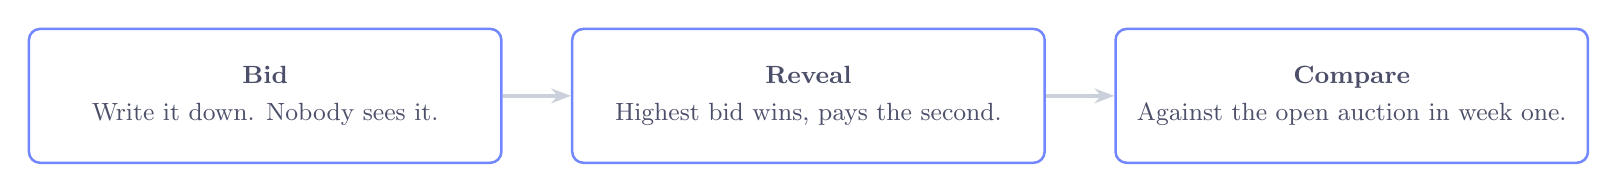
\begin{tikzpicture}[font=\small]
      \stepbox{s0}{0.0}{\textbf{Bid}\\[0.25em]
        Write it down. Nobody sees it.}
      \stepbox{s1}{6.9}{\textbf{Reveal}\\[0.25em]
        Highest bid wins, pays the second.}
      \stepbox{s2}{13.8}{\textbf{Compare}\\[0.25em]
        Against the open auction in week one.}
      \draw[-{Stealth[length=2.5mm]}, inkfaint, line width=1.2pt] (s0) -- (s1);
      \draw[-{Stealth[length=2.5mm]}, inkfaint, line width=1.2pt] (s1) -- (s2);
    \end{tikzpicture}

    \vspace{2.4em}

    {\large On sale: a five pound note. What is it worth to you?}}

\newpage
\slidehead{The bids}

\vspace{0.5cm}

\hspace{0.3cm}
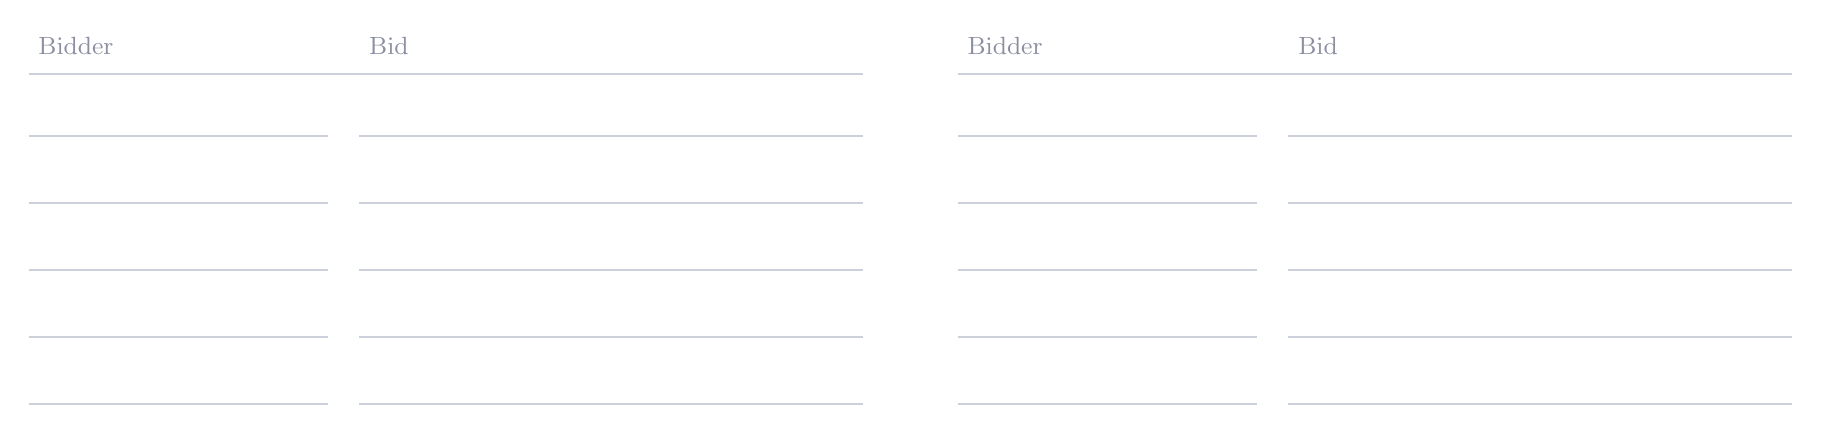
\begin{tikzpicture}[font=\small]
  \foreach \lab/\col in {Bidder/0, Bid/4.2, Bidder/11.8, Bid/16.0}{%
    \node[anchor=west, text=inkgrey] at (\col,0) {\lab};}
  \draw[inkfaint, line width=0.7pt] (0,-0.36) -- (10.6,-0.36);
  \draw[inkfaint, line width=0.7pt] (11.8,-0.36) -- (22.4,-0.36);
  \foreach \row in {1,2,3,4,5}{%
    \foreach \shift in {0,11.8}{%
      \draw[inkfaint, line width=0.7pt]
        (\shift,-0.85*\row-0.3) -- (\shift+3.8,-0.85*\row-0.3);
      \draw[inkfaint, line width=0.7pt]
        (\shift+4.2,-0.85*\row-0.3) -- (\shift+10.6,-0.85*\row-0.3);}}
\end{tikzpicture}

\vspace{0.7cm}

{\large Winner \blank[3.4] \hspace{1.4cm} Highest bid \blank[2.2]
\hspace{1.4cm} Price paid \blank[2.2] \hspace{1.4cm} Their profit
\blank[2.2]}

\newpage
\slidehead{What are the rules, exactly?}

\vspace{1cm}

{\large Everyone submits \underline{\hspace{4cm}}, without seeing anyone
else's.}

\vspace{1.1cm}

{\large The item goes to \underline{\hspace{5cm}}.}

\vspace{1.1cm}

{\large The winner pays \underline{\hspace{5cm}}.}

\vspace{1.4cm}

{\large In week one we ran this open and ascending, and it went badly. Name one
thing that changed when we sealed it:}

\vspace{0.6cm}

\hspace*{1cm}\blank[8]

\newpage
\slidehead{Should you bid what it is worth?}

\vspace{0.5cm}

{\large Your value is \(v\). Let \(b\) be the highest bid among everybody else.
Compare bidding \(v\) with bidding something else.}

\vspace{0.7cm}

\begin{minipage}[t]{0.47\linewidth}
\raggedright
{\large\bfseries You bid above your value}

\vspace{0.5em}

{\large You only win extra times when \(b\) is between \blank[1.4] and
\blank[1.4], and then you pay \blank[1.4] and make \blank[1.4].}

\vspace{0.8em}

\workspace{10.6}{3.4}
\end{minipage}
\hfill
\begin{minipage}[t]{0.47\linewidth}
\raggedright
{\large\bfseries You bid below your value}

\vspace{0.5em}

{\large You lose some auctions you would have won, and when you do still win
you pay \blank[3.4].}

\vspace{0.8em}

\workspace{10.6}{3.4}
\end{minipage}

\vspace{0.6cm}

{\large So bidding your true value is \underline{\hspace{5cm}}.}

\newpage
\slidehead{Why that matters}

\vspace{1.1cm}

{\large If truth is a weakly dominant strategy, then to bid well you need to
know \underline{\hspace{5cm}} about the other bidders.}

\vspace{1.3cm}

{\large So the seller gets the item to the person who
\underline{\hspace{5cm}}, which is not guaranteed otherwise.}

\vspace{1.3cm}

{\large Now change one rule: the winner pays their \emph{own} bid. Is truth
still weakly dominant? \blank[2.2] \hspace{1.4cm} What should you do instead?
\blank[5]}

\vspace{1cm}

\begin{center}
\workspace{22.6}{2.4}
\end{center}

\newpage
\slidehead{The same thing, as an exam answer}

\vspace{0.5cm}

{\large What we just did in the room is \textbf{Question 1} on the Auctions
page, with values \(v_1 = 10\), \(v_2 = 7\) and \(v_3 = 4\).}

\vspace{0.9cm}

\hspace{0.6cm}
\begin{minipage}{0.92\linewidth}
{\large
\begin{tabbing}
\hspace{1.2cm} \= \hspace{17cm} \= \kill
\textbf{(a)} \> The rules of a second-price (Vickrey) auction. \> [3]\\[0.55em]
\textbf{(b)} \> With truthful bids: the winner, the price and the
  payoff. \> [3]\\[0.55em]
\textbf{(c)} \> Show bidding \(v_1 = 10\) is weakly dominant, above and
  below. \> [7]\\[0.55em]
\textbf{(d)} \> Why that is a desirable property. \> [4]\\[0.55em]
\textbf{(e)} \> Would truth still be weakly dominant in a first-price
  auction? \> [2]
\end{tabbing}}
\end{minipage}

\vspace{1.2cm}

\begin{center}
{\large\color{inkgrey} vknight.org/gt/topics/auctions.html}
\end{center}

\end{document}
